% 固定来源PDF第4页第26题：椭圆、双曲线焦点与动点 P 的关系。
% 取 a=1.6 仅用于示意绘图，满足 a>=sqrt(2)；没有把该数值加入题面条件。
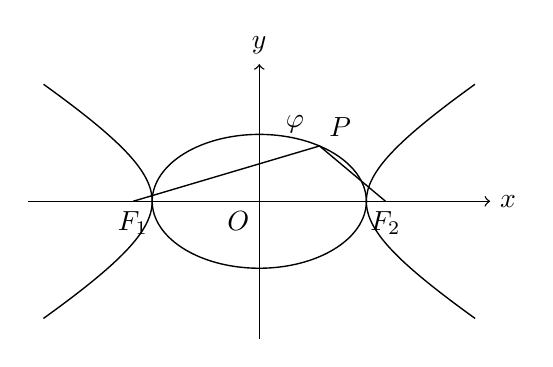
\begin{tikzpicture}[line width=.5pt,x=.85cm,y=.85cm]
  \pgfmathsetmacro{\a}{1.6}
  \pgfmathsetmacro{\f}{sqrt(\a*\a+1)}
  \pgfmathsetmacro{\py}{sqrt(1-(.9/\a)^2)}
  \coordinate (O) at (0,0);
  \coordinate (F1) at (-\f,0);
  \coordinate (F2) at (\f,0);
  \coordinate (P) at (.9,\py);
  \draw[->] (-3.45,0)--(3.45,0) node[right] {$x$};
  \draw[->] (0,-2.05)--(0,2.05) node[above] {$y$};
  \draw[domain=0:360,samples=150,smooth]
    plot ({\a*cos(\x)},{sin(\x)});
  \draw[domain=-1.75:1.75,samples=100,smooth]
    plot ({\a*sqrt(1+\x*\x)},\x);
  \draw[domain=-1.75:1.75,samples=100,smooth]
    plot ({-\a*sqrt(1+\x*\x)},\x);
  \draw (F1)--(P)--(F2);
  \node[below left] at (O) {$O$};
  \node[below] at (F1) {$F_1$};
  \node[below] at (F2) {$F_2$};
  \node[above right] at (P) {$P$};
  \node[above left,xshift=-2pt,yshift=1pt] at (P) {$\varphi$};
\end{tikzpicture}
